\documentclass[12pt]{article}

\usepackage[T1]{fontenc}
\usepackage{polski}
\usepackage[utf8]{inputenc}
\usepackage{graphicx} % Include images.
\usepackage{float} % Force turning off float for figures.
\graphicspath{ {images/} }
\usepackage{listings}
\lstset{language=sql}
\usepackage{color}

\topmargin -1.0cm
\oddsidemargin 0.2cm
\textwidth 16cm
\textheight 22cm
\footskip 1.0cm


\title{Baza danych „Konferencje”}

\author
{\Large{Marcin Aman, Tomasz Czajęcki}\\
\\
\large{Podstawy Baz Danych}\\
\normalsize{\bf Dr Inż. Lech Siwik}\\
\normalsize{\it Informatyka na wydziale Informatyki, Elektroniki i Telekomunikacji}\\
}
  %https://my.vertabelo.com/model/cxdCDtoTzbwnwRLfrf5LsR8ycdLzANym
  %https://www.overleaf.com/12584034bkmfxkbfvjvf#/47959726/
	%Add conference day -> sprawdzenie czy jest w datach okreslonych przez konferencje.
  %add_order_item - czy przepelni sie dzien konferencji lub tez workshop
  %add_workshop_participant powinno zliczac czy nie ma zbyt dużo osob w order itemsach
  %return payment? Nie warto sprawdzic czy ktos sie nie zarejestrowal z tego orderid?
  %update workshop information - sprawdzenie czy nie ma juz wiekszej ilosci miejsc niz updatowana
  %Change workshop time - zablokowanie manipulacji pomiedzy dniami.
  %cancel order - realizacja zwrotu
  %get_customers_with_not_filled_participants ? Co z tym?
  %too_few_places_on_workshop_to_order moze informacja ile jest dost? Mamy na to funkcje.

\begin{document}

\maketitle

\newpage

\section{Wstęp}
Celem projektu jest realizacja bazy danych, która będzie używana przez firmę organizującą konferencje. Klienci tej firmy (osoby prywatne jak i firmy) mogą utworzyć zamówienie na poszczególne dni oraz odbywające się w tym czasie warsztaty. Mogą to być wydarzenia darmowe jak i też płatne. Cena konferencji jest zależna w głównej mierze od terminu oraz jest możliwa do obniżenia poprzez zniżkę studencką. Klient musi dostarczyć do 2 tygodni listę uczestników danego wydarzenia.
\section{Diagram bazy danych}
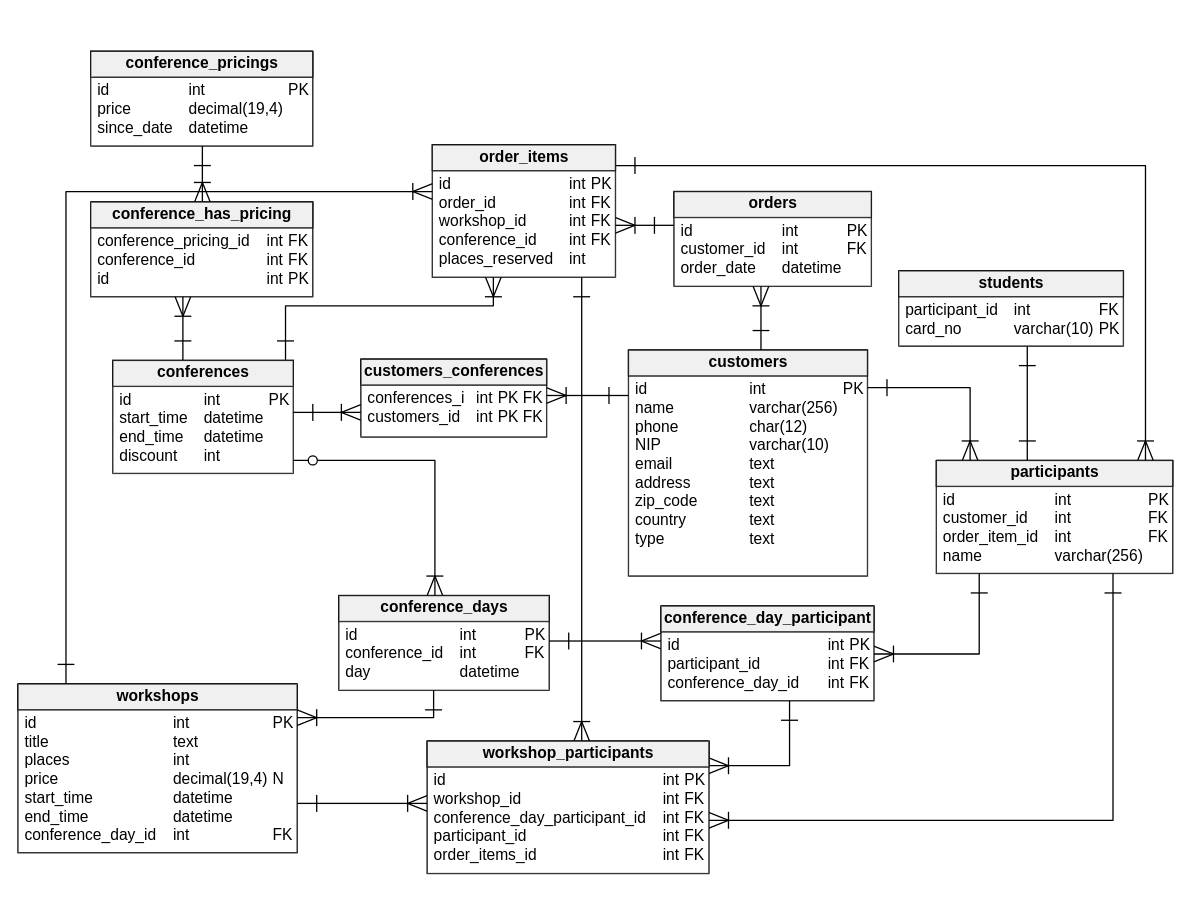
\includegraphics[width=\textwidth]{ConferenceSchema.png}
\section{Opis bazy}
\paragraph{Customers \newline}
Tabela przechowuje informację o Klientach. Klientami mogą być zarówno osoby prywatne jak i firmy. Klienci indeksowani są poprzez ID. Dodatkowo posiadają w systemie nazwę. W przypadku firm jest nazwa firmy a dla osób prywatnych w tym polu jest dostępne imię oraz nazwisko. Co więcej, dostepne tam są inne informacje potrzebne do kontaktu oraz obsługi zamówień danego Klienta jak numer telefonu, numer NIP, email, adress. Ostatnim polem jest tutaj informacja o typie Klienta. Może to być firma lub osoba prywatna.
\begin{lstlisting}
CREATE TABLE customers (
	id INT identity NOT NULL,
	name varchar(256) NOT NULL,
	phone char(12),
	NIP varchar(10),
	email TEXT,
	address TEXT,
	zip_code TEXT,
	country TEXT,
	is_company bit NULL,
	CONSTRAINT customers_pk PRIMARY KEY (id)
);

\end{lstlisting}
\paragraph{Orders\\}
\noindent
Informuje o wszystkich zamówieniach jakie widnieją w systemie. Zarówno aktualnie realizowane jak i realizowane. \newline \newline
\textit{id} - identyfikator danego zamówienia \newline
\textit{customer\_id} - identyfikator Klienta, który utworzył dane zamówienie \newline
\textit{order\_date} - data złożenia zamówienia \newline
\textit{is\_cancelled} - informacja, czy zamówienie jest anulowane. \\

\begin{lstlisting}
CREATE TABLE orders (
	id INT identity NOT NULL,
	customer_id INT NOT NULL,
	order_date DATETIME NOT NULL,
	is_cancelled bit NULL,
	CONSTRAINT orders_pk PRIMARY KEY (id)
);
\end{lstlisting}
\paragraph{Order\_items \newline}
Tabela przedstawia zawartość zamówień. Znajdziemy tam informacje o danej konferencji poprzez identyfikator oraz warsztatów prowadzonych podczas niej. \newline \newline
\textit{id} - identyfikator danej zwartości zamówienia \newline
\textit{order\_id} - identyfikator zamówienia powiązanego z danym elementem \newline
\textit{workshop\_id} - identyfikator warsztatów, które zostały zamówione \newline
\textit{placesReserved} - ilość miejsc jakie są dostępne na danym warsztacie. \newline

\begin{lstlisting}
CREATE TABLE order_items (
	id INT identity NOT NULL,
	order_id INT NOT NULL,
	workshop_id INT NOT NULL,
	places_reserved INT NOT NULL,
	conference_days_id INT NOT NULL,
	CONSTRAINT order_items_pk PRIMARY KEY (id)
);
\end{lstlisting}

\paragraph{payments \\}
Tabela przechowuje dane o płatnościach za zamówienia. Umożliwia też księgowanie zwrotów, które są oznaczane ujemną wartością kwoty. \\ \\
\textit{id} - identyfikator danej transakcji \\
\textit{value} - kwota na którą opiewa \\
\textit{order\_id} - identyfikator zakupu do za który została wniesiona \\
\begin{lstlisting}
CREATE TABLE payments (
	id INT identity NOT NULL,
	value DECIMAL(8,2) NULL,
	order_id INT NOT NULL,
	CONSTRAINT Payments_pk PRIMARY KEY (id)
);
\end{lstlisting}
\paragraph{conferences \newline}
Informuje o wszystkich detalach na temat konferencji. \newline \newline
\textit{id} - identyfikator danej konferencji \newline
\textit{name} - krótka nazwa konferencji \\
\textit{start\_time} - czas rozpoczęcia konferencji. \newline
\textit{end\_time} - czas zakończenia konferencji. \newline
\textit{discout} - pole informujące o zniżce jaka przysługuje na daną konferencję. \newline
\begin{lstlisting}
CREATE TABLE conferences (
	id INT identity NOT NULL,
	[name] varchar(50),
	start_time DATETIME NOT NULL,
	end_time DATETIME NOT NULL,
	discount NUMERIC(2,2) NOT NULL,
	CONSTRAINT conferences_pk PRIMARY KEY (id)
);

\end{lstlisting}

\paragraph{customers\_conference\_days\\}
Tabela przechowuje dane na temat powiązania Klientów z poszczególnymi dniami konferencji. Umożliwia to zapisanie się jednego Klienta na więcej niż 1 dzień konferencji.\\ \\
\textit{Customer\_id} - identyfikator Klienta \\
\textit{conference\_days\_id} - identyfikator poszczególnego dnia konferencji.
\begin{lstlisting}
CREATE TABLE customers_conference_days (
	customer_id INT NOT NULL,
	conference_days_id INT NOT NULL,
	CONSTRAINT customers_conference_days_pk PRIMARY KEY (customer_id,conference_days_id)
);
\end{lstlisting}

\paragraph{conference\_pricing \newline}
Informuje o danych przedziałach cenowych na konferencje. Cena jest zależna od daty złożenia zamówienia oraz daty poszczególnej konferencji.\newline \newline
\textit{id} - identyfiakator kwoty \newline
\textit{price} - wartość kwoty za poszczególnego uczestnika danej konferencji. Jest to wartość za uczestnika, który nie korzysta ze zniżki studneckiej.\newline
\textit{dates\_since} - data od której dana cena obowiązuje.
\begin{lstlisting}
CREATE TABLE conference_pricing (
    id int  NOT NULL,
    price decimal(19,4)  NOT NULL,
    since_date datetime  NOT NULL,
    CONSTRAINT conference_pricing_pk PRIMARY KEY  (id)
);
\end{lstlisting}

\paragraph{conference\_has\_pricing \newline}
Tabela przechowuje dane o powiązaniach konferencji z danymi przedziałami czasowymi, za czym idzie również kwota pojedynczego biletu.
Z racji tego jest możliwa rezerwacja miejsc w różnym czasie. \newline
\textit{id} - identyfikator główny.
\textit{conference\_pricing\_id} - identyfikator rekordu z tabeli ConferencePricing. Przechowuje on informację o kwocie oraz jej zależności od przedziału czasu. \newline
\textit{conferences\_id} - identyfikator konferencji. \\
\begin{lstlisting}
CREATE TABLE conference_has_pricing (
	id INT identity NOT NULL,
	conference_pricing_id INT NOT NULL,
	conference_id INT NOT NULL,
	CONSTRAINT conference_has_pricing_pk PRIMARY KEY (id)
);
\end{lstlisting}


\paragraph{conference\_days \newline}
Przechwuje informacje o danym dniu konfernencji. Jedna konfernecja może mieć wiele dni i podczas nich wiele warsztatów. \newline \newline
\textit{id} - identyfikator danego dnia konferencji. \newline
\textit{conference\_id} - klucz identyfikacyjny konferencji do której należy dany dzień. \newline
\textit{day} - dzień konferencji \newline
\textit{seats} - ilość miejsc jaka jest dostępna podczas poszczególnego dnia konferencji.\\ \\
\begin{lstlisting}
CREATE TABLE conference_days (
	id INT identity NOT NULL,
	conference_id INT NOT NULL,
	day DATETIME NOT NULL,
	seats INT NULL,
	CONSTRAINT conference_days_pk PRIMARY KEY (id)
);
\end{lstlisting}
\paragraph{conference\_day\_participant \newline}
Informuje o uczestnikach danej konferencji. Do ich identyfikacji potrzebne jest wyszczególnienie ich imienia oraz nazwiska oraz informacja o firmie z której pochodzą. \newline \newline
\textit{Participant\_id} - identyfikator uczestnika z wszystkich uczestników wszystkich dni konfernecji. \newline
\textit{Conference\_Days\_id} - identyfikator konferencji na którą jest zarejestrowany \newline
\textit{participant\_id} - identyfikator uczestnika \newline
\begin{lstlisting}
CREATE TABLE conference_day_participant (
	id INT identity NOT NULL,
	participant_id INT NOT NULL,
	conference_day_id INT NOT NULL,
	CONSTRAINT conference_day_participant_pk PRIMARY KEY (id)
);
 \end{lstlisting}
\paragraph{participants \newline}
Informuje o uczestnikach oraz przechowuje ich dane. \newline \newline
\textit{id} - identyfikator uczestnika.\newline
\textit{Customer\_id} - identyfikator firmy od której pochodzi ten uczestnik \newline
\textit{Name} - Imię oraz nazwisko uczestnika \newline
\textit{Order\_Items\_ID} - identyfikator elementu zamówienia z którego pochodzi dany uczestnik.\\
\textit{card\_no} - jeśli uczestnik jest studentem odnajdziemy tutaj numer jego legitymacji. Jest to wartość unikalna i indywidualna dla każdej osoby.
\begin{lstlisting}
CREATE TABLE participants (
	id INT identity NOT NULL,
	customer_id INT NOT NULL,
	order_item_id INT NOT NULL,
	name varchar(256) NOT NULL,
	card_no INT unique,
	CONSTRAINT participants_pk PRIMARY KEY (id)
);
\end{lstlisting}
\paragraph{workshops \newline}
Przechowuje informaje o warsztatach jakie są prowadzone podczas poszczególnych dni konferencji. W ramach jednej konferencji może być wiele warsztatów, część z nich jest płatna.\newline \newline
\textit{id} - identyfikator warsztatu \newline
\textit{Title} - nazwa warsztatu \newline
\textit{Places} - ilość miejsc jakie są dostępne podczas warsztatu \newline
\textit{Price} - kwota bazowa za jedno miejsce. \newline
\textit{Start\_time} - czas rozpoczęcia warsztatu \newline
\textit{End\_time} - czas zakończenia warsztatu \newline
\textit{Conference\_days\_id} - identyfikator dnia konferencji w ramach której warsztat się odbywa \newline
\begin{lstlisting}
CREATE TABLE workshops (
	id INT identity NOT NULL,
	conference_day_id INT NOT NULL,
	title TEXT NOT NULL,
	places INT NOT NULL,
	price DECIMAL(8,2) NULL,
	start_time DATETIME NOT NULL,
	end_time DATETIME NOT NULL,
	CONSTRAINT workshops_pk PRIMARY KEY (id)
);

\end{lstlisting}

\section{Procedury}
\subsection{Procedury dodające \\}
\paragraph{create\_conference \\}
Procedura umożliwia dodanie konferencji. Potrzebna jest jej nazwa, czas oraz ewentualna zniżka jaka jest planowana. \\ \\
\begin{lstlisting}
 CREATE PROCEDURE [dbo].[create_conference] (
  @name NVARCHAR(127),
  @start_time DATETIME,
  @end_time DATETIME,
  @discount DECIMAL(2,2),
  @conference_id INT = NULL OUT
) AS BEGIN
  SET NOCOUNT ON;

  BEGIN TRY
    BEGIN TRANSACTION;
      IF @name IS NULL OR LTRIM(@name) = ''
        THROW 50000, '@name is NULL or empty', 1
	  IF @start_time >= @end_time
		THROW 50000, '@start_time is later or equal than @end_time', 1
	  IF @start_time <= GETDATE()
		THROW 50000, '@start_time is from past' , 1

      INSERT INTO conferences (
				[name],
				start_time,
				end_time,
				discount
			) VALUES (
				@name,
				@start_time,
				@end_time,
				@discount
			)
      SET @conference_id = SCOPE_IDENTITY()
    COMMIT TRANSACTION;
  END TRY
  BEGIN CATCH
    ROLLBACK TRANSACTION;
    THROW
  END CATCH
END
GO
\end{lstlisting}
\newpage
\paragraph{create\_workshop\\}
Procedura dodaje warsztat do danego dnia konferencji. Potrzebne jest wprowadzenie identyfikatora dnia konferencji, nazwy, ilości miejsc oraz czasu. \\
\begin{lstlisting}
 CREATE PROCEDURE [dbo].[create_workshop]
		@conference_day_id INT,
		@title varchar(256),
		@places INT,
		@price DECIMAL(8,2),
		@start_time DATETIME,
		@end_time DATETIME
	AS BEGIN

	BEGIN TRY
	BEGIN TRANSACTION;
	IF @start_time >= @end_time
		THROW 50000, '@start_time is later or equal than @end_time', 1
	IF @start_time < GETDATE()
		THROW 50000, '@start_time is from past', 1
	IF @price < 0
		THROW 50000, '@price is lower than 0', 1
	IF @places <= 0
		THROW 50000, '@seats are lower or equal 0', 1
	IF NOT EXISTS (
       SELECT * FROM conference_days
       WHERE conference_days.conference_id = @conference_day_id
    	)
		THROW 50000, '@Conference_day not found', 1

		INSERT INTO workshops(
			conference_day_id,
			title,
			places,
			price,
			start_time,
			end_time
		) VALUES (
			@conference_day_id,
			@title,
			@places,
			@price,
			@start_time,
			@end_time
		)
		COMMIT TRANSACTION
	END TRY
	BEGIN CATCH
		ROLLBACK TRANSACTION;
		THROW
	END CATCH
END
GO
\end{lstlisting}
\newpage
\paragraph{add\_customer \\}
Procedura dodaje Klienta do bazy danych. Przy okazji sprawdza, czy posiadamy kontakt z danym Klientem. Pola email oraz phone mogą być null-ami ale przynajmniej jedno z nich musi być uzupełnione. Dodatkowo nazwa Klienta musi być wypełniona. \\
\begin{lstlisting}
CREATE PROCEDURE [dbo].[add_customer]
	@name varchar(256),
	@phone char(9),
	@NIP char(10),
	@email TEXT,
	@adress TEXT,
	@zip_code TEXT,
	@county TEXT,
	@is_company bit
AS BEGIN
	BEGIN TRY
	BEGIN TRANSACTION
	IF (@phone is null) AND (@email is null)
		THROW 50000, '@phone and @email is null.
        No contact with customer', 1
	IF @name is null or LTRIM(@name) = ''
		THROW 50000, '@name is null or empty', 1
	INSERT INTO customers (
		[name],
		phone,
		NIP,
		email,
		address,
		zip_code,
		country,
		is_company
	) VALUES (
		@name,
		@phone,
		@NIP,
		@email,
		@adress,
		@zip_code,
		@county,
		@is_company
	)
	COMMIT TRANSACTION
	END TRY
	BEGIN CATCH
		ROLLBACK TRANSACTION;
		THROW
	END CATCH
END
GO

\end{lstlisting}
\newpage
\paragraph{add\_conference\_day \\}
Procedura dodaje dni konferencji. Potrzebne jest aby konferencja już istniała przed dodaniem dnia gdyż potrzebujemy jej ID. Procedura sprawdza, czy dana konferencja jest w bazie, dodatkowo chroni przed dodawaniem duplikatów w postaci 2 dni konferencji w tym samym terminie do jednej konferencji. \\
\begin{lstlisting}
CREATE PROCEDURE [dbo].[add_conference_day]
	@conference_id INT,
	@day DATETIME,
	@places INT
AS BEGIN
	BEGIN TRY
	BEGIN TRANSACTION
	IF NOT EXISTS (SELECT * FROM conferences
       			WHERE id = @conference_id)
	THROW 50000, '@conference_id is invalid. No such conference', 1
	IF @day < GETDATE()
	THROW 50000, '@date is from past', 1
	IF EXISTS (SELECT id FROM conference_days
          WHERE conference_id = @conference_id AND [day] = @day)
	THROW 50000, 'Conference already in database', 1
	IF @places <= 0
	THROW 50000, '@places are lower or equal 0', 1

	INSERT INTO conference_days (
		conference_id,
		[day],
		seats
	) VALUES (
		@conference_id,
		@day,
		@places
	)
	COMMIT TRANSACTION
	END TRY
	BEGIN CATCH
		ROLLBACK TRANSACTION;
			THROW
		END CATCH
END
GO
\end{lstlisting}
\newpage
\paragraph{add\_order \\}
Procedura dodająca nowe zamówienie. Przed jej realizacją potrzebujemy mieć utworzonego Klienta w bazie. Dodatkowo wprowadza ona do bazy datę złożenia, jest ona później potrzebna do policzenia kwoty biletu. Przy tworzeniu nowego zamówienia standardowo jest pole is\_cancelled jest ustawiane na 0.\\
\begin{lstlisting}
CREATE PROCEDURE [dbo].[add_order]
	@customer_id INT,
	@order_date DATETIME
AS BEGIN
	BEGIN TRY
	BEGIN TRANSACTION
	IF NOT EXISTS (SELECT * FROM customers
       				WHERE id = @customer_id)
	THROW 50000, '@customer_id not in database', 1

	INSERT INTO orders (
		customer_id,
		order_date,
		is_cancelled
	) VALUES (
		@customer_id,
		@order_date,
		0
	)
	COMMIT TRANSACTION
	END TRY
	BEGIN CATCH
		ROLLBACK TRANSACTION;
			THROW
		END CATCH
END
GO

\end{lstlisting}
\newpage

\paragraph{add\_order\_item \\}
Procedura dodająca szczegóły danego zamówienia do tabeli order items. Wcześniej dane zamówienie musi zostać utworzone w systemie. Dodaje informacje na temat danego dnia konferencji oraz warsztatów na jakie dany Klient chciałby wykupić miejsca. Jednocześnie sprawdza, czy na danym warsztacie jest wystarczająca ich ilość oraz, czy nie przepełni to ilości przeznaczonej na dany dzień konferencji. \\
\begin{lstlisting}
CREATE PROCEDURE [dbo].[add_order_item]
	@order_id INT,
	@workshop_id INT,
	@conference_day_id INT,
	@places_reserved INT
AS BEGIN
	BEGIN TRY
	BEGIN TRANSACTION
	IF NOT EXISTS (SELECT * FROM orders WHERE id = @order_id)
		THROW 50000, '@order_id not in database', 1
	IF NOT EXISTS (SELECT * FROM conference_days
    				WHERE id = @conference_day_id)
		THROW 50000, '@conference_day_id not in database', 1
	IF NOT EXISTS (SELECT * FROM workshops WHERE id = @workshop_id)
		THROW 50000, '@workshop not in database', 1
	IF @places_reserved <= 0
		THROW 50000, '@places_reserved below or equal 0', 1
	INSERT INTO order_items (
		order_id,
		workshop_id,
		conference_days_id,
		places_reserved
	) VALUES (
		@order_id,
		@workshop_id,
		@conference_day_id,
		@places_reserved
	)
	COMMIT TRANSACTION
	END TRY
	BEGIN CATCH
		ROLLBACK TRANSACTION;
		THROW
	END CATCH
END
GO


\end{lstlisting}
\newpage
\paragraph{add\_participants \\}
Procedura dodaje uczestnika do bazy. Jest on związany z określonym Klientem poprzez identyfikator, tak samo jak z order\_item-em. \\
\begin{lstlisting}
CREATE PROCEDURE [dbo].[add_participants]
	@customer_id INT,
	@order_item_id INT,
	@name varchar(256)
AS BEGIN
	BEGIN TRY
		BEGIN TRANSACTION
		IF NOT EXISTS (SELECT * FROM customers WHERE id = @customer_id)
			THROW 50000, '@customer_id not in database', 1
		IF NOT EXISTS (SELECT * FROM order_items WHERE id = @order_item_id)
			THROW 50000, '@order_item not in database', 1
		IF LTRIM(@name) = ''
			THROW 50000, '@name is empty', 1
		IF (
			SELECT count(id) FROM participants
			WHERE order_item_id = @order_item_id
		) >= (
			SELECT places_reserved FROM order_items
			WHERE id = @order_item_id
		)
			THROW 50000, 'No more places left in this order_item', 1

		INSERT INTO participants (
			customer_id,
			order_item_id,
			[name]
		) VALUES (
			@customer_id,
			@order_item_id,
			@name
		)
		COMMIT TRANSACTION
	END TRY
	BEGIN CATCH
		ROLLBACK TRANSACTION;
		THROW
	END CATCH
END
GO
\end{lstlisting}
\newpage
\paragraph{add\_student\_participant\\}
Analogicznie jak poprzednia procedura dodaje ona uczestnika, jednakże jest on studentem. W poprzednim przypadku pole card\_no zostało automatycznie wypełnione wartością null. Jeśli chcemy dodać studenta jest wymagane, aby został podany numer legitymacji. \\
\begin{lstlisting}
CREATE PROCEDURE [dbo].[add_student_participant]
	@customer_id INT,
	@order_item_id INT,
	@name varchar(256),
	@card_no INT
AS BEGIN
	BEGIN TRY
	BEGIN TRANSACTION
	IF NOT EXISTS (SELECT * FROM customers WHERE id = @customer_id)
		THROW 50000, '@customer_id not in database', 1
	IF NOT EXISTS (SELECT * FROM order_items WHERE id = @order_item_id)
		THROW 50000, '@order_item not in database', 1
	IF LTRIM(@name) = ''
		THROW 50000, '@name is empty', 1
	IF (
		SELECT count(id) FROM participants
		WHERE order_item_id = @order_item_id
	) >= (
		SELECT places_reserved FROM order_items
		WHERE id = @order_item_id
	)
		THROW 50000, 'No more places left in this order_item', 1
		INSERT INTO participants (
			customer_id,
			order_item_id,
			[name],
			card_no
		) VALUES (
			@customer_id,
			@order_item_id,
			@name,
			@card_no
		)
	COMMIT TRANSACTION
	END TRY
	BEGIN CATCH
		ROLLBACK TRANSACTION;
		THROW
	END CATCH
END
GO
\end{lstlisting}
\newpage
\paragraph{add\_workshop\_participant\\}
Procedura dodająca uczestnika danego warsztatu. Aby było to możliwe potrzebne jest zarejestrowanie na dany dzień konferencji i podanie identyfikatora uczestnika dnia konferencji, ogólnego identyfikatora danej osoby oraz numeru z order\_items, który umożliwiłby stwierdzenie, że jeszcze zostały miejsca z zamówienia.\\
\begin{lstlisting}
CREATE PROCEDURE [dbo].[add_workshop_participant]
	@workshop_id INT,
	@conference_day_participant_id INT,
	@participant_id INT,
	@order_item_id INT
AS BEGIN
	BEGIN TRY
	BEGIN TRANSACTION
	IF (
		SELECT count(id) FROM workshop_participants
		WHERE workshop_id = @workshop_id
	) >= (
		SELECT places FROM workshops
		WHERE id = @workshop_id
	)
		THROW 50000, 'No more places left in this workshop', 1
	IF (
		SELECT count(wp.id) FROM workshop_participants AS wp
		INNER JOIN conference_day_participant AS cdp
        on wp.conference_day_participant_id = cdp.id
		INNER JOIN participants AS p on p.id = cdp.participant_id
		WHERE p.id = @participant_id
		) >= (
		SELECT places_reserved FROM order_items
		WHERE id = @order_item_id
	)
		THROW 50000, 'No more places left available in this order', 1

		INSERT INTO workshop_participants (
			workshop_id,
			conference_day_participant_id
		) VALUES (
			@workshop_id,
			@conference_day_participant_id
		)
	COMMIT TRANSACTION
	END TRY
	BEGIN CATCH
		ROLLBACK TRANSACTION;
		THROW
	END CATCH
END
GO
\end{lstlisting}
\newpage
\paragraph{add\_payment \\}
Procedura dodająca płatność. Ważne jest aby każda płatność była za konkretne zamówienie, z racji tego przechowujemy identyfikator.\\
\begin{lstlisting}
CREATE PROCEDURE [dbo].[add_payment]
	@value DECIMAL(8,2),
	@order_id INT
AS BEGIN
	BEGIN TRY
	BEGIN TRANSACTION
	IF NOT EXISTS (SELECT id FROM orders WHERE id = @order_id)
		THROW 50000, '@order_id not in database', 1
	INSERT INTO payments (
		[value],
		orders_id
	) VALUES (
		@value,
		@order_id
	)
	COMMIT TRANSACTION
	END TRY
	BEGIN CATCH
		ROLLBACK TRANSACTION;
		THROW
	END CATCH
END
GO

\end{lstlisting}
\newpage
\paragraph{add\_conference\_day\_participant\\}
Procedura dodaje uczestnika na dany dzień konferencji. Przy okazji sprawdza, czy jest on w bazie oraz czy przypadkiem nie jest już zapisany na dany dzień konferencji.\\
\begin{lstlisting}
CREATE PROCEDURE [dbo].[add_conference_day_participant]
	@participant_id INT,
	@conference_day_id INT
AS BEGIN
	BEGIN TRY
	BEGIN TRANSACTION
	IF NOT EXISTS (SELECT id FROM participants
    				WHERE id = @participant_id)
		THROW 50000, '@participant_id not in database' ,1
	IF NOT EXISTS (SELECT id FROM conference_days
    				WHERE id = @conference_day_id)
		THROW 50000, '@conference_day_id not in database' ,1
	IF EXISTS (SELECT id FROM conference_day_participants
    WHERE participant_id = @participant_id AND
    conference_day_id = @conference_day_id)
		THROW 50000, 'Participant already enrolled for this conference day',1

	INSERT INTO conference_day_participants (
		conference_day_id,
		participant_id
	) VALUES (
		@conference_day_id,
		@participant_id
	)
	COMMIT TRANSACTION
	END TRY
	BEGIN CATCH
		ROLLBACK TRANSACTION;
		THROW
	END CATCH
END
GO
\end{lstlisting}
\newpage
\paragraph{add\_conference\_pricing \\}
Prodcedura dodaje wartość do tabeli Conference\_pricing. Przy okazji sprawdza, czy podana wartość nie jest mniejsza niż 0. \\
\begin{lstlisting}
CREATE PROCEDURE [dbo].[add_conference_pricing]
	@price DECIMAL(8,2),
	@since_date DATETIME
AS BEGIN
	BEGIN TRY
	BEGIN TRANSACTION
	IF @price < 0
		THROW 50000, '@price is lower than 0',1

	INSERT INTO conference_pricings (
		price,
		since_date
	) VALUES (
		@price,
		@since_date
	)
	COMMIT TRANSACTION
	END TRY
	BEGIN CATCH
		ROLLBACK TRANSACTION;
		THROW
	END CATCH
END
GO

\end{lstlisting}
\newpage

\paragraph{add\_conference\_has\_pricing\\}
Procedura dodaje połączenie pomiędzy Conference\_Pricing a Conferences. Przed wprowadzeniem danych do bazy sprawdzane jest, czy Conference\_ID oraz Conference\_Pricing\_ID są obecne w bazie. \\
\begin{lstlisting}
CREATE PROCEDURE [dbo].[add_conference_has_pricing]
	@conference_pricing_id INT,
	@conference_id INT
AS BEGIN
	BEGIN TRY
	BEGIN TRANSACTION
	IF NOT EXISTS (SELECT id FROM conferences
    				WHERE id = @conference_id)
		THROW 50000, '@conference_id not in database',1
	IF NOT EXISTS (SELECT id FROM conference_pricings
    				WHERE id = @conference_pricing_id)
		THROW 50000, '@conference_pricing_id not in database',1

	INSERT INTO conference_has_pricing (
		conference_id,
		conference_pricing_id
	) VALUES (
		@conference_id,
		@conference_pricing_id
	)
	COMMIT TRANSACTION
	END TRY
	BEGIN CATCH
		ROLLBACK TRANSACTION;
		THROW
	END CATCH
END
GO

\end{lstlisting}
\newpage

\paragraph{update\_customer\_data \\}
Procedura zmienia dane Klienta. Przed wykonaniem tej czynności sprawdzane są warunki poprawności danych takie jak: istnieje identyfikatora Klienta, poprawne pole name oraz czy posiadamy jakikolwiek kontakt z Klientem. \\
\begin{lstlisting}
CREATE PROCEDURE [dbo].[update_customer_data]
	@customer_id INT,
	@name VARCHAR(256),
	@phone CHAR(9),
	@NIP char(10),
	@email TEXT,
	@address TEXT,
	@zip_code TEXT,
	@county TEXT,
	@is_company bit
AS BEGIN
	BEGIN TRY
	BEGIN TRANSACTION
	IF NOT EXISTS (SELECT * FROM customers WHERE id = @customer_id)
		THROW 50000, 'Customer not in database', 1
	IF (@phone is null) AND (@email is null)
		THROW 50000, '@phone and @email is null.
        			Customer must provide a contact method', 1
	IF @name is null or LTRIM(@name) = ''
		THROW 50000, '@name is null or empty', 1
	UPDATE customers
		SET [name] = @name,
			phone = @phone,
			NIP = @NIP,
			email = @email,
			address = @address,
			zip_code = @zip_code,
			country =  @county,
			is_company = @is_company
		WHERE customers.id = @customer_id
	COMMIT TRANSACTION
	END TRY
	BEGIN CATCH
		ROLLBACK TRANSACTION;
		THROW
	END CATCH
END
GO

\end{lstlisting}
\newpage

\paragraph{delete\_customer \\}
Procedura usuwa dane Klienta z bazy. Jest to możliwe jedynie, gdy nie posiada żadnych zakupów w historii lub też aktywnych. \\
\begin{lstlisting}
CREATE PROCEDURE [dbo].[delete_customer]
	@customer_id INT
AS BEGIN
	BEGIN TRY
	BEGIN TRANSACTION
	IF EXISTS (SELECT * FROM orders WHERE customer_id = @customer_id)
		THROW 50000, 'Customer data cannot be removed, an order was made', 1

	DELETE customers
		WHERE id = @customer_id
	COMMIT TRANSACTION
	END TRY
	BEGIN CATCH
		ROLLBACK TRANSACTION;
		THROW
	END CATCH
END
GO

\end{lstlisting}
\newpage

\paragraph{delete\_conference\_pricing \\}
Procedura usuwa dany rekord z tabeli Conference\_Pricing. Jest to możliwe jedynie, gdy nie używa go żadna konferencja.\\
\begin{lstlisting}
CREATE PROCEDURE [dbo].[delete_conference_pricing]
	@conference_pricing_id INT
AS BEGIN
	BEGIN TRY
	BEGIN TRANSACTION
	IF EXISTS (SELECT * FROM conference_has_pricing
    WHERE conference_pricing_id = @conference_pricing_id)

    THROW 50000, 'Conference pricing is used by conference.', 1

	DELETE conference_pricings
		WHERE id = @conference_pricing_id
	COMMIT TRANSACTION
	END TRY
	BEGIN CATCH
		ROLLBACK TRANSACTION;
		THROW
	END CATCH
END
GO
\end{lstlisting}
\newpage

\paragraph{return\_payment \\}
Procedura pozwala na zrealizowanie zwrotu płatności za dane zamówienie. Przed jego wykonaniem jest sprawdzane, czy takowy nie miał już miejsca. \\
\begin{lstlisting}
CREATE PROCEDURE [dbo].[return_payment]
	@payment_id INT
AS BEGIN
	BEGIN TRY
	BEGIN TRANSACTION
	IF NOT EXISTS (SELECT * FROM payments WHERE id = @payment_id)
		THROW 50000, 'Payment not found', 1
	DECLARE @value DECIMAL(8,2)
	SET @value = (SELECT [value]*(-1) FROM payments
    						WHERE id = @payment_id)

	DECLARE @order_id INT
	SET @order_id = (SELECT orders_id FROM payments
    						WHERE id = @payment_id)

	IF EXISTS (SELECT * FROM payments
    		WHERE orders_id = @order_id AND [value] < 0)
		THROW 50000, 'Money was already returned', 1

	INSERT INTO payments(
		[value],
		orders_id
	) VALUES (
		@value,
		@order_id
	)
	COMMIT TRANSACTION
	END TRY
	BEGIN CATCH
		ROLLBACK TRANSACTION;
		THROW
	END CATCH
END
GO
\end{lstlisting}
\newpage

\paragraph{update\_workshop\_information\\}
Procedura umożliwiająca zamianę parametrów danego warsztatu. Do dyspozycji mamy zmianę tytułu, ilości miejsc oraz ceny. Przed zmianą ilości miejsc sprawdzane jest czy już nie mamy większej ilości zarezerwowanej. \\
\begin{lstlisting}
CREATE PROCEDURE [dbo].[update_workshop_information]
	@workshop_id INT,
	@title VARCHAR(256),
	@places INT,
	@price DECIMAL(8,2)
AS BEGIN
	BEGIN TRY
	BEGIN TRANSACTION
	IF NOT EXISTS (SELECT * FROM workshops WHERE id = @workshop_id)
		THROW 50000, 'Workshop not found', 1
	IF LTRIM(@title) = ''
		THROW 50000, 'Title is empty', 1
	IF @places <= 0
		THROW 50000, 'Places are lower or equal 0', 1
	IF @price < 0
		THROW 50000, 'Price is lower than 0', 1

	UPDATE workshops
		SET	title = @title,
			places = @places,
			price = @price
		WHERE id = @workshop_id
	COMMIT TRANSACTION
	END TRY
	BEGIN CATCH
		ROLLBACK TRANSACTION;
		THROW
	END CATCH
END
GO
\end{lstlisting}
\newpage

\paragraph{change\_workshop\_time \\}
Możliwa jest też zmiana czasu w którym odbywa się dany warsztat, jednakże nie może być na niego wtedy zapisana ani jedna osoba. \\
\begin{lstlisting}
CREATE PROCEDURE [dbo].[change_workshop_time]
	@workshop_id INT,
	@startTime DATETIME,
	@endTime DATETIME
AS BEGIN
	BEGIN TRY
	BEGIN TRANSACTION
	IF NOT EXISTS (SELECT * FROM workshops WHERE id = @workshop_id)
		THROW 50000, 'Workshop not found',1
	IF @startTime >= @endTime
		THROW 50000, 'Start time is later than endtime',1
	IF day(@startTime) != day(@endTime)
		THROW 50000, 'Begining and end days have to be the same',1
	IF EXISTS (SELECT * FROM order_items WHERE id = @workshop_id)
		THROW 50000, 'There is at least 1 person enrolled'
        'for this workshop. Can change the time',1

	UPDATE workshops
		SET start_time = @startTime,
			end_time = @endTime
			WHERE id = @workshop_id

	COMMIT TRANSACTION
	END TRY
	BEGIN CATCH
		ROLLBACK TRANSACTION;
		THROW
	END CATCH
END
GO
\end{lstlisting}
\newpage

\paragraph{cancel\_order\\}
Procedura umożliwia usuwanie zamówień. Dodatkowo usuwa uczestników jacy wynikają z jego treści.
\begin{lstlisting}
CREATE PROCEDURE [dbo].[cancel_order]
	@order_id INT
AS BEGIN
	BEGIN TRY
	BEGIN TRANSACTION
	IF NOT EXISTS (SELECT * FROM orders WHERE id = @order_id)
		THROW 50000, 'Order not in database', 1
	UPDATE orders
		SET is_cancelled = 1
		WHERE id = @order_id

	DECLARE @orderItemID INT
	SET @orderItemID = (SELECT id FROM order_items WHERE
    					order_id = @order_id)

	DELETE conference_day_participants
		WHERE id IN (
		SELECT cdp.id FROM conference_day_participants AS cdp
		INNER JOIN workshop_participants AS wp ON
           		wp.conference_day_participant_id = cdp.id
		INNER JOIN order_items AS oi ON oi.id = @orderItemID
           		AND oi.workshop_id = wp.workshop_id
		)

	DELETE workshop_participants
		WHERE id in (SELECT wp.id FROM workshop_participants AS wp
		INNER JOIN conference_day_participant AS cdp on
        		wp.conference_day_participant_id = cdp.id
		INNER JOIN participants AS p on p.id = cdp.participant_id
		WHERE p.order_item_id in
		(SELECT oi.id FROM order_items AS oi
		INNER JOIN orders AS o on o.id = oi.order_id
		WHERE o.id = @order_id))

	COMMIT TRANSACTION
	END TRY
	BEGIN CATCH
		ROLLBACK TRANSACTION;
		THROW
	END CATCH
END
GO
\end{lstlisting}
\newpage
\section{Funkcje}
\paragraph{does\_workshops\_overlap\\}
Funkcja sprawdza czy 2 warsztaty nachodzą na siebie. \\
\begin{lstlisting}
CREATE FUNCTION [dbo].[does_workshops_overlap](@workshop_id1 INT, @workshop_id2 INT) RETURNS BIT
AS BEGIN
DECLARE
	@startTime1 DATETIME,
	@startTime2 DATETIME,
	@endTime1 DATETIME,
	@endTime2 DATETIME
SET @startTime1 = (SELECT start_time FROM workshops WHERE id = @workshop_id1)
SET @startTime2 = (SELECT start_time FROM workshops WHERE id = @workshop_id2)
SET @endTime1 = (SELECT end_time FROM workshops WHERE id = @workshop_id1)
SET @endTime2 = (SELECT end_time FROM workshops WHERE id = @workshop_id2)

IF ((@startTime1 < @startTime2 AND @endTime2 > @endTime1)
	OR (@startTime2 > @startTime1 AND @endTime2 < @endTime1)
	OR (@startTime2 < @startTime1 AND @endTime2 < @endTime1))
	RETURN 1

RETURN 0
END
GO
\end{lstlisting}
\newpage

\paragraph{get\_free\_day\_places \\}
Funkcja zwraca informację na temat ilości miejsc jakie są wolne w danym dniu konferencji. Informacje pobiera z tabeli order\_items. \\
\begin{lstlisting}
CREATE FUNCTION [dbo].[get_free_day_places] (@conference_day_id INT)
RETURNS INT
AS BEGIN
RETURN (
	SELECT seats FROM conference_days WHERE id = @conference_day_id
	) - (
	SELECT sum(oi.places_reserved) FROM order_items AS oi
	INNER JOIN orders AS o on o.id = oi.order_id AND o.is_cancelled=0
	INNER JOIN workshops AS w on w.id = oi.workshop_id
	WHERE w.conference_day_id = @conference_day_id
)
END
GO
\end{lstlisting}

\paragraph{get\_free\_workshop\_seats \\}
Funkcja zwraca wartość miejsc, które są wolne na danym warsztacie. Analogicznie jak poprzednia informacje czerpie z tabeli order\_items. \\
\begin{lstlisting}
CREATE FUNCTION [dbo].[get_free_workshop_seats] (@workshop_id INT)
RETURNS INT
AS BEGIN
RETURN (
	SELECT places FROM workshops WHERE id = @workshop_id
	) - (
	SELECT count(*) FROM order_items AS oi
	INNER JOIN orders AS o ON oi.order_id = o.id AND o.is_cancelled = 0
	WHERE workshop_id = @workshop_id
);
END
GO
\end{lstlisting}
\newpage

\paragraph{get\_conference\_day\_participants \\}
Procedura zwraca tabelę identyfikatorów uczestnika oraz imion Klientów, którzy zapisali się na dany dzień konferencji. \\
\begin{lstlisting}
CREATE FUNCTION [dbo].[get_conference_day_participants]
(@ConferenceDayID INT) RETURNS TABLE
AS
RETURN (
	SELECT part.id, [name] FROM participants AS part
	INNER JOIN conference_day_participant ON participant_id = part.id
	WHERE conference_day_id = @ConferenceDayID
);
GO
\end{lstlisting}

\paragraph{get\_workshop\_participants \\}
Procedura zwraca tabelę uczestników danego warsztatu. Analogicznie jak poprzednio są tą pola identyfikatora uczestnika oraz imię. \\
\begin{lstlisting}
CREATE FUNCTION [dbo].[get_workshop_participants] (@workshopID INT)
RETURNS TABLE
AS
RETURN (
  SELECT [name],part.id FROM participants AS part
  INNER JOIN conference_day_participant AS cdpart
  	ON cdpart.participant_id = part.id
  INNER JOIN workshop_participants AS wp
  	ON wp.conference_day_participant_id = cdpart.id
  INNER JOIN workshops AS w ON w.id = wp.workshop_id
  WHERE w.id = @workshopID
);
GO
\end{lstlisting}\
\newpage
\section{Triggery}
\paragraph{too\_few\_places\_on\_workshop\_to\_order\\}
Trigger blokuje możliwość dodania nowego zamówienia na warsztat, jeśli brakuje na niego miejsc. \\
\begin{lstlisting}
CREATE TRIGGER [dbo].[too_few_places_on_workshop_to_order]
ON [dbo].[order_items]
AFTER INSERT, UPDATE
AS BEGIN
	DECLARE @workshop_id INT
	SET @workshop_id = (SELECT workshop_id FROM inserted)

	DECLARE @seats INT
	SET @seats = (SELECT places FROM workshops WHERE id = @workshop_id)

	IF(
		SELECT sum(places_reserved) FROM order_items AS oi
		INNER JOIN orders AS o ON o.id = oi.order_id
        	AND o.is_cancelled = 0
		WHERE workshop_id = @workshop_id
	) + (SELECT places_reserved FROM inserted) > @seats
		THROW 50000, 'Too few places on workshop',1
END
GO
\end{lstlisting}
\newpage

\paragraph{too\_few\_places\_on\_conference\_day\_on\_order\\}
Trigger blokuje możliwość utworzenia zamówienia, jeśli w danym dniu konferencji brakuje miejsc.\\
\begin{lstlisting}
CREATE TRIGGER [dbo].[too_few_places_on_conference_day_on_order]
ON [dbo].[order_items]
AFTER INSERT,UPDATE
AS BEGIN
	DECLARE @ConferenceDayID INT
	SET @ConferenceDayID = (
		SELECT cd.id FROM conference_days AS cd
		INNER JOIN workshops AS w on w.conference_day_id = cd.id
		INNER JOIN inserted AS i on i.workshop_id = w.id
	)
	IF dbo.get_free_day_places(@ConferenceDayID) < (SELECT places_reserved FROM inserted)
		THROW 50000, 'Too few places on conference day',1
END
GO
\end{lstlisting}
\newpage

\paragraph{already\_enrolled\_on\_other\_workshop \\}
Trigger uniemożliwia jednemu uczestnikowi uczestnictwo w więcej niż 1 warsztacie prowadzonym w jednym czasie.\\
\begin{lstlisting}
CREATE TRIGGER [dbo].[already_enrolled_on_other_workshop]
ON [dbo].[workshop_participants]
AFTER INSERT, UPDATE
AS BEGIN
DECLARE @workshop_id INT
DECLARE @conference_day_participant_id INT
SET @workshop_id = (SELECT workshop_id FROM inserted)
SET @conference_day_participant_id = (SELECT conference_day_participant_id FROM inserted)

IF EXISTS (SELECT * FROM workshops AS w
	WHERE dbo.does_workshops_overlap(@workshop_id,w.id) = 1 AND @workshop_id <> w.id
)
	THROW 50000, 'Participant already enrolled for another workshop at the same time',1
END
GO

\end{lstlisting}
\newpage

\paragraph{}
\begin{lstlisting}

\end{lstlisting}
\newpage

\paragraph{}
\begin{lstlisting}

\end{lstlisting}
\newpage

\paragraph{}
\begin{lstlisting}

\end{lstlisting}
\newpage


\end{document}